\documentclass[xcolor=table]{beamer}

\usepackage{booktabs}
\usepackage{amsmath, amssymb}
\usepackage{graphicx}
\usepackage{tikz}
\usetikzlibrary{shapes.geometric, arrows.meta, positioning, calc}
\usepackage{colortbl}

\mode<presentation> {
    \usetheme{Madrid}
}

\setbeamertemplate{caption}[numbered]
\setbeamertemplate{navigation symbols}{}

% COLOR DEFINITIONS (NIT Meghalaya Palette)
\definecolor{myblue}{RGB}{24, 116, 205}     % NITM Dodger Blue
\definecolor{mydarkblue}{RGB}{0, 43, 91}    % Dark Navy Blue
\definecolor{mqgray}{RGB}{55, 58, 54}
\definecolor{mqlightgray}{RGB}{242, 244, 247}
\definecolor{highlightgreen}{RGB}{34, 139, 34}
\definecolor{accentcrimson}{RGB}{178, 34, 34}

\usecolortheme[named=myblue]{structure}

% Header and Footer Styling
\setbeamercolor{title in head/foot}{bg=mqlightgray, fg=mqgray}
\setbeamercolor{author in head/foot}{bg=myblue, fg=white}
\setbeamercolor{page number in head/foot}{bg=mydarkblue, fg=white}

\makeatletter
\setbeamertemplate{footline}{
  \leavevmode%
  \hbox{%
  \begin{beamercolorbox}[wd=.45\paperwidth,ht=2.25ex,dp=1ex,center]{author in head/foot}%
    \usebeamerfont{author in head/foot}\insertshortauthor~(\insertshortinstitute)
  \end{beamercolorbox}%
  \begin{beamercolorbox}[wd=.45\paperwidth,ht=2.25ex,dp=1ex,center]{title in head/foot}%
    \usebeamerfont{title in head/foot}\insertshorttitle
  \end{beamercolorbox}%
  \begin{beamercolorbox}[wd=.10\paperwidth,ht=2.25ex,dp=1ex,center]{page number in head/foot}%
    \usebeamerfont{page number in head/foot}\insertframenumber{} / \inserttotalframenumber 
  \end{beamercolorbox}}%
  \vskip0pt%
}
\makeatother

% TITLE AND METADATA
\title[Multi-Source Media Lineage Retrieval]{Multi-Source Lineage Retrieval in Composite Media with Dynamic Token Alignment and Importance Gating}

\author[Vivek Negi -- T25CS012]{Vivek Negi \\ \small Roll No: T25CS012}

\institute[NIT Meghalaya]{
  \textit{Under the guidance of}\\
  \textbf{Dr. Akhilendra Pratap Singh}\\[0.15cm]
  \IfFileExists{pictures/NIT logo.jpeg}{%
    \includegraphics[scale=0.16]{pictures/NIT logo.jpeg}\\[0.1cm]%
  }{%
    
\begin{tikzpicture}
      \node[draw=myblue, fill=mqlightgray, rounded corners=2pt, inner sep=3pt] {
        \scriptsize\textbf{\textcolor{mydarkblue}{NATIONAL INSTITUTE OF TECHNOLOGY MEGHALAYA}}
      };
    \end{tikzpicture}\\[0.15cm]
  }%
  Department of Computer Science and Engineering\\
  National Institute of Technology Meghalaya\\
  Shillong, India
}
\date{\today}

\begin{document}

% ==============================================================================
% SLIDE 1: TITLE PAGE
% ==============================================================================
\begin{frame}
  \titlepage
\end{frame}

% ==============================================================================
% SLIDE 2: INTRODUCTION
% ==============================================================================
\begin{frame}{Introduction: What is Composite Media Lineage?}
  \begin{itemize}
    \item \textbf{Traditional Copy Detection:} Search engines like Google Lens or TinEye look for exact copies or lightly edited duplicates of a \textit{single} image.
    \item \textbf{The Composite Problem:} In the real world, manipulated media usually takes parts from \textbf{two or more different images}:
    \begin{itemize}
      \item \textbf{Parent A (Background):} The main scene or landscape.
      \item \textbf{Parent B (Donor):} An object (car, person, animal) cut from another photo.
    \end{itemize}
    \item \textbf{Our Goal:} Build a system that takes a composite query and searches a gallery of thousands of photos to find \textbf{both Parent A and Parent B}.
    \item \textbf{Why it matters:} Copyright protection, fake news verification, and digital evidence investigation.
  \end{itemize}
\end{frame}

% ==============================================================================
% SLIDE 3: PROBLEM STATEMENT
% ==============================================================================
\begin{frame}{The Core Problem: Background Dominance}
  \begin{block}{Why Existing AI Models Fail on Composites}
    Existing vision models compress the entire image into a single global vector.
  \end{block}
  \vspace{0.2cm}
  \begin{itemize}
    \item \textbf{The Background Wins:} Because the background covers $70\%\text{--}85\%$ of the image, the AI focuses almost entirely on the background. It finds Parent A with $100\%$ accuracy.
    \item \textbf{The Donor is Lost:} The smaller donor object (covering only $15\%\text{--}35\%$) is completely ignored by the global vector, causing donor recall to fail.
    \item \textbf{Rigid Grids Cut Objects in Half:} Cutting an image into fixed $2\times2$ or $3\times3$ squares chops objects placed in the center into four pieces, destroying their shape.
    \item \textbf{No Retraining Allowed:} Retraining giant models (ResNets/ViTs) is too expensive and causes them to forget general features. We must solve this with a lightweight approach.
  \end{itemize}
\end{frame}

% ==============================================================================
% SLIDE 4: LITERATURE REVIEW 1 - SSCD (CVPR 2022)
% ==============================================================================
\begin{frame}{Literature Review: Meta SSCD (CVPR 2022)}
  \textbf{Paper:} \textit{A Self-Supervised Descriptor for Image Copy Detection} \\
  \textbf{Authors:} E. Pizzi, S. Durasamy, S. Couprie, M. Douze, A. Gordo (Meta AI)
  \vspace{0.2cm}
  \begin{itemize}
    \item \textbf{What it does:} 
    \begin{itemize}
      \item Meta AI trained a ResNet-50 on millions of images using self-supervised contrastive learning specifically for copy detection.
      \item Produces a compact, 512-dimensional visual fingerprint for any image.
    \end{itemize}
    \item \textbf{Why it is strong:} 
    \begin{itemize}
      \item Highly robust against heavy JPEG compression, color changes, and crops.
      \item Currently the gold-standard backbone for image retrieval benchmarks.
    \end{itemize}
    \item \textbf{Limitation for our task:} 
    \begin{itemize}
      \item It was designed for single images. On composites, its global pooling is blind to small, localized pasted objects.
    \end{itemize}
  \end{itemize}
\end{frame}

% ==============================================================================
% SLIDE 5: LITERATURE REVIEW 2 - TRUFOR (CVPR 2023)
% ==============================================================================
\begin{frame}{Literature Review: TruFor (CVPR 2023)}
  \textbf{Paper:} \textit{TruFor: Leveraging All-Round Clues for Trustworthy Forgery Detection} \\
  \textbf{Authors:} F. Guillaro, D. Cozzolino, A. Sud, N. Dufour, L. Verdoliva
  \vspace{0.2cm}
  \begin{itemize}
    \item \textbf{What it does:} 
    \begin{itemize}
      \item Uses computer vision to inspect subtle camera sensor noise, compression traces, and lighting inconsistencies across image pixels.
      \item Outputs a heatmap showing exactly which part of an image was forged.
    \end{itemize}
    \item \textbf{Why it is strong:} 
    \begin{itemize}
      \item Best-in-class performance at localizing spliced boundaries.
    \end{itemize}
    \item \textbf{Limitation for our task:} 
    \begin{itemize}
      \item \textbf{Detection is not Attribution:} TruFor can tell you \textit{"this car was pasted into the photo"}, but it \textbf{cannot find the source file} the car came from. It has no gallery search capability.
    \end{itemize}
  \end{itemize}
\end{frame}

% ==============================================================================
% SLIDE 6: LITERATURE REVIEW 3 - CHEN ET AL. (APRIL 2024)
% ==============================================================================
\begin{frame}{Literature Review: Single Simple Patch Network (2024)}
  \textbf{Paper:} \textit{A Single Simple Patch is All You Need for AI-generated Image Detection} \\
  \textbf{Authors:} Jiaxuan Chen, Jieteng Yao, Li Niu (arXiv:2402.01123, April 2024)
  \vspace{0.2cm}
  \begin{itemize}
    \item \textbf{What it does:} 
    \begin{itemize}
      \item Discovered that image generators (GANs, Diffusion) focus heavily on generating complex textures, while neglecting authentic camera sensor noise in simple/smooth patches.
      \item Extracts noise fingerprints from just \textbf{a single simple patch} using high-pass filters to distinguish real images from AI fakes.
    \end{itemize}
    \item \textbf{Why it connects to our work:} 
    \begin{itemize}
      \item Proves that \textbf{local patch-level evidence} carries vital forensic clues that global image representations discard.
    \end{itemize}
    \item \textbf{Limitation for our task:} 
    \begin{itemize}
      \item It is strictly a binary classifier (Real vs. Fake). It cannot trace multi-parent lineages or search an image gallery for source assets.
    \end{itemize}
  \end{itemize}
\end{frame}

% ==============================================================================
% SLIDE 7: LITERATURE REVIEW 4 - AIGIBENCH (NEURIPS 2025)
% ==============================================================================
\begin{frame}{Literature Review: AIGIBench (NeurIPS 2025)}
  \textbf{Paper:} \textit{Is Artificial Intelligence Generated Image Detection a Solved Problem?} \\
  \textbf{Authors:} Ziqiang Li, Jiazhen Yan, Ziwen He, Kai Zeng, et al. (NeurIPS 2025)
  \vspace{0.2cm}
  \begin{itemize}
    \item \textbf{What it does:} 
    \begin{itemize}
      \item The latest comprehensive benchmark evaluating 11 state-of-the-art detectors across 23 modern generative subsets (SDXL, FLUX, Midjourney-v6, DALLE-3).
      \item Reveals that existing detectors experience massive failure drops when applied to in-the-wild content and face-swaps.
    \end{itemize}
    \item \textbf{Key Insight That Validates Our Method:} 
    \begin{itemize}
      \item In Section 3.4, they proved that **resizing an image destroys forensic details**, whereas **cropping preserves fine-grained local structures and high frequencies**.
      \item This directly justifies our proposed **Dynamic Cropping/Slicing strategy** over global resized representations!
    \end{itemize}
  \end{itemize}
\end{frame}

% ==============================================================================
% SLIDE 8: PROPOSED ARCHITECTURE
% ==============================================================================
\begin{frame}{Proposed Architecture}
  \centering
  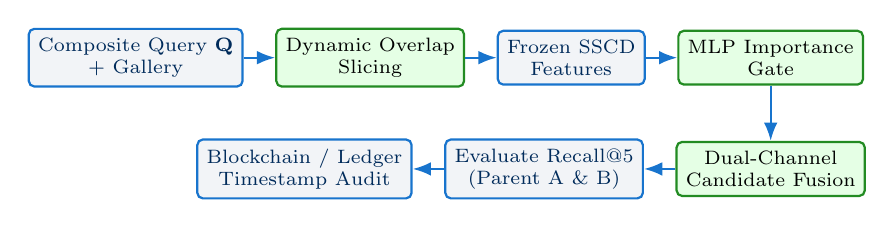
\begin{tikzpicture}[
    node distance=0.6cm and 0.4cm,
    every node/.style={font=\scriptsize, align=center},
    box/.style={rectangle, draw=myblue, fill=mqlightgray, rounded corners=2pt, minimum height=0.6cm, minimum width=1.5cm, text=mydarkblue, thick},
    proc/.style={rectangle, draw=highlightgreen, fill=green!10, rounded corners=2pt, minimum height=0.6cm, minimum width=1.6cm, text=black, thick},
    arrow/.style={-Latex, thick, myblue}
  ]
    \node[box] (query) {Composite Query $\mathbf{Q}$\\+ Gallery};
    \node[proc, right=of query] (slicing) {Dynamic Overlap\\Slicing};
    \node[box, right=of slicing] (encoder) {Frozen SSCD\\Features};
    \node[proc, right=of encoder] (gate) {MLP Importance\\Gate};
    \node[proc, below=0.7cm of gate] (ranking) {Dual-Channel\\Candidate Fusion};
    \node[box, left=of ranking] (eval) {Evaluate Recall@5\\(Parent A \& B)};
    \node[box, left=of eval] (ledger) {Blockchain / Ledger\\Timestamp Audit};

    \draw[arrow] (query) -- (slicing);
    \draw[arrow] (slicing) -- (encoder);
    \draw[arrow] (encoder) -- (gate);
    \draw[arrow] (gate) -- (ranking);
    \draw[arrow] (ranking) -- (eval);
    \draw[arrow] (eval) -- (ledger);
  \end{tikzpicture}
  \vspace{0.3cm}
  \begin{block}{Three Simple Steps}
    \begin{enumerate}
      \item \textbf{Extract Smart Patches:} Use center crops and overlapping windows so no donor object gets cut in half.
      \item \textbf{Weight by Importance:} A tiny 2-layer neural network learns to highlight the donor patch and ignore repetitive background.
      \item \textbf{Dual Channel Search:} Search for Parent A using the whole image, and Parent B using the weighted patches.
    \end{enumerate}
  \end{block}
\end{frame}

% ==============================================================================
% SLIDE 9: DYNAMIC OVERLAPPING SLICING
% ==============================================================================
\begin{frame}{Methodology: Dynamic Overlapping Slicing}
  \begin{columns}[T]
    \begin{column}{0.52\textwidth}
      \textbf{The Problem with Rigid Grids:}
      \begin{itemize}
        \item Cutting an image into a rigid $2\times2$ grid splits centered objects into 4 pieces.
        \item SSCD cannot recognize one-quarter of a dog or a car.
      \end{itemize}
      \vspace{0.2cm}
      \textbf{Our Dynamic Slicing Solution:}
      \begin{itemize}
        \item \textbf{Center Anchors:} We add crops centered at $50\%$ and $66\%$ scale. This guarantees that centered objects are captured in one whole piece.
        \item \textbf{Overlapping Windows:} We slide local windows with a $33\%$ overlap, ensuring objects on boundaries are never chopped.
      \end{itemize}
    \end{column}
    \begin{column}{0.45\textwidth}
      \centering
      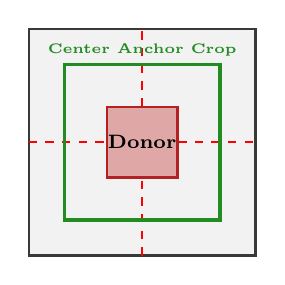
\begin{tikzpicture}[scale=0.9]
        \draw[thick, draw=mqgray, fill=gray!10] (0,0) rectangle (3.2,3.2);
        \draw[dashed, red, thick] (1.6,0) -- (1.6,3.2);
        \draw[dashed, red, thick] (0,1.6) -- (3.2,1.6);
        \draw[fill=accentcrimson!40, draw=accentcrimson, thick] (1.1,1.1) rectangle (2.1,2.1);
        \node at (1.6, 1.6) {\scriptsize \textbf{Donor}};
        \draw[draw=highlightgreen, very thick] (0.5, 0.5) rectangle (2.7, 2.7);
        \node[highlightgreen] at (1.6, 2.9) {\tiny \textbf{Center Anchor Crop}};
      \end{tikzpicture}
      \vspace{0.1cm}
      {\centering\scriptsize \textbf{Figure:} Center anchor capturing donor intact.\par}
    \end{column}
  \end{columns}
\end{frame}

% ==============================================================================
% SLIDE 10: LEARNED IMPORTANCE GATE
% ==============================================================================
\begin{frame}{Methodology: Learned MLP Importance Gate}
  \begin{itemize}
    \item \textbf{The Idea:} Not all patches are equally useful. Background patches are repetitive (sky, grass, road) and already match Parent A. We need the model to pay attention to the spliced donor.
    \item \textbf{How it works:}
    \begin{itemize}
      \item We feed each patch embedding into a tiny 2-layer neural network (MLP).
      \item The MLP assigns an \textbf{importance weight between 0 and 1} to each patch.
      \item Patches containing the donor object get high weights ($\approx 0.45$), while background patches get near zero.
    \end{itemize}
    \item \textbf{Fast \& Lightweight:}
    \begin{itemize}
      \item Contains less than \textbf{70,000 parameters}.
      \item Trains in under 1 minute on a free GPU without touching or fine-tuning the heavy foundation model.
    \end{itemize}
  \end{itemize}
\end{frame}

% ==============================================================================
% SLIDE 11: EXPERIMENTAL SETUP
% ==============================================================================
\begin{frame}{Experimental Setup}
  \begin{itemize}
    \item \textbf{100\% Real Photographs:} Used real-world natural images from the official MS-COCO 2017 dataset (people, vehicles, animals, indoor/outdoor scenes).
    \item \textbf{Gallery Database:} 1,000 unindexed natural photos acting as the search space.
    \item \textbf{Composite Queries:} 300 realistic photographic composites created with Gaussian edge blending (donor size controlled between $15\%\text{--}35\%$).
    \item \textbf{Data Splits:} $70\%$ Training (210 queries), $15\%$ Validation (45 queries), and $15\%$ Held-Out Test (45 queries).
    \item \textbf{Hardware:} NVIDIA Tesla T4 GPU running on cloud environment.
    \item \textbf{Primary Metric:} \textbf{Full Lineage Recall@5} (Did the top 5 results contain BOTH Parent A and Parent B?).
  \end{itemize}
\end{frame}

% ==============================================================================
% SLIDE 12: RESULTS & ABLATION STUDY
% ==============================================================================
\begin{frame}{Experimental Results (Held-Out Test Set)}
  \begin{center}
  \renewcommand{\arraystretch}{1.25}
  \footnotesize
  \begin{tabular}{|l|c|c|c|c|}
    \hline
    \textbf{Method} & \textbf{Parent A} & \textbf{Parent B} & \textbf{Full Lineage} & \textbf{Latency} \\ \hline \hline
    Global SSCD Baseline & 100.00\% & 51.11\% & 51.11\% & \textbf{193 ms} \\ \hline
    Uniform Local (Rigid $2\times2, 3\times3$) & 100.00\% & 53.33\% & 53.33\% & 2277 ms \\ \hline
    \textbf{Uniform Local (Dynamic Overlap)} & 100.00\% & \textbf{75.56\%} & \textbf{75.56\%} & 2117 ms \\ \hline
    SSCD + MLP Gate (Rigid) & 100.00\% & 82.22\% & 82.22\% & 2265 ms \\ \hline
    \rowcolor{green!15}
    \textbf{SSCD + MLP Gate (Dynamic) [Ours]} & \textbf{100.00\%} & \textbf{88.89\%} & \textbf{88.89\%} & 2125 ms \\ \hline
  \end{tabular}
  \end{center}
  \vspace{0.15cm}
  \begin{block}{Key Takeaways}
    \begin{itemize}
      \item \textbf{Global baseline misses half the donors:} Achieves only $51.11\%$ full lineage.
      \item \textbf{Dynamic slicing gives an instant $+22.23\%$ leap:} Proves that boundary crossing was the main reason rigid grids failed.
      \item \textbf{Proposed system achieves $88.89\%$:} Near 9 out of 10 composites have both source parents retrieved in the top 5!
    \end{itemize}
  \end{block}
\end{frame}

% ==============================================================================
% SLIDE 13: DISCUSSION OF RESULTS
% ==============================================================================
\begin{frame}{Discussion: Why Did Our Method Work So Well?}
  \begin{itemize}
    \item \textbf{1. Dynamic Slicing Fixed Object Cutting ($+22.23\%$ gain):}
    \begin{itemize}
      \item By simply introducing center-anchors and overlapping crops, the donor object is always captured in full in at least one crop.
    \end{itemize}
    \vspace{0.1cm}
    \item \textbf{2. The Gate Filtered Out Background Clutter ($+13.33\%$ gain):}
    \begin{itemize}
      \item Background patches (sky, ground) generated false matches with other gallery images.
      \item The MLP gate assigned near-zero weight to these clutter patches and focused search attention strictly on the donor object.
    \end{itemize}
    \vspace{0.1cm}
    \item \textbf{3. Background Accuracy Remained at 100\%:}
    \begin{itemize}
      \item By keeping a dedicated global channel for Parent A, we never sacrificed background recall while hunting for the donor.
    \end{itemize}
  \end{itemize}
\end{frame}

% ==============================================================================
% SLIDE 14: FUTURE WORK - BLOCKCHAIN INTEGRATION
% ==============================================================================
\begin{frame}{Future Work: Blockchain-Audited Media Lineage}
  \begin{itemize}
    \item \textbf{Why Blockchain?} Visual AI can retrieve candidate images, but cannot legally prove which image was created first. A malicious user can claim their composite is the original.
    \item \textbf{On-Chain Hash Notarization:}
    \begin{itemize}
      \item When a creator takes a photo, its SHA-256 visual hash is recorded onto an immutable blockchain (e.g., Polygon / Ethereum).
      \item Gives each photo an unalterable, tamper-proof timestamp.
    \end{itemize}
    \item \textbf{Smart Contract Provenance Auditing:}
    \begin{itemize}
      \item A smart contract verifies the lineage condition:
      $$\text{Timestamp}(\text{Parent A}) < \text{Timestamp}(\text{Query}) \;\land\; \text{Timestamp}(\text{Parent B}) < \text{Timestamp}(\text{Query})$$
      \item If verified, the smart contract automatically settles copyright attribution or licensing royalties between creators.
    \end{itemize}
  \end{itemize}
\end{frame}

% ==============================================================================
% SLIDE 15: CONCLUSION & KEY REFERENCES
% ==============================================================================
\begin{frame}{Conclusion \& Key References}
  \textbf{Summary of Contributions:}
  \begin{itemize}
    \item Solved the \textbf{Background Dominance Paradox} in multi-source image attribution without retraining heavy vision backbones.
    \item Dynamic overlapping tokenization resolved boundary cuts, boosting recall by $+22\%$.
    \item Our lightweight MLP gate achieved \textbf{$88.89\%$ Full Lineage Recall@5} on real photos.
  \end{itemize}
  \vspace{0.15cm}
  \textbf{Key References:}
  \scriptsize
  \begin{enumerate}
    \item E. Pizzi et al., ``A Self-Supervised Descriptor for Image Copy Detection,'' \textit{CVPR}, 2022.
    \item F. Guillaro et al., ``TruFor: Leveraging All-Round Clues for Forgery Detection,'' \textit{CVPR}, 2023.
    \item J. Chen, J. Yao, L. Niu, ``A Single Simple Patch is All You Need for AI-generated Image Detection,'' \textit{arXiv:2402.01123}, 2024.
    \item Z. Li, J. Yan, Z. He, K. Zeng, et al., ``Is Artificial Intelligence Generated Image Detection a Solved Problem? (AIGIBench),'' \textit{NeurIPS}, 2025.
  \end{enumerate}
  \vspace{0.2cm}
  \centering
  \small \textbf{\textcolor{myblue}{Thank You! Questions \& Discussion}}
\end{frame}

\end{document}